%Weihnachtsblatt, Aufgabe 1
%Dorkenwald,Soloninov 

% !TEX program = pdflatex
% !TEX encoding = UTF-8 Unicode
% !TEX spellcheck = de_DE

\documentclass[convert={density=300,size=1080x800,outext=.png}]{standalone}

\usepackage[utf8]{inputenc}
\usepackage[T1]{fontenc}
\usepackage{lmodern}

\usepackage{tikz}

\begin{document}
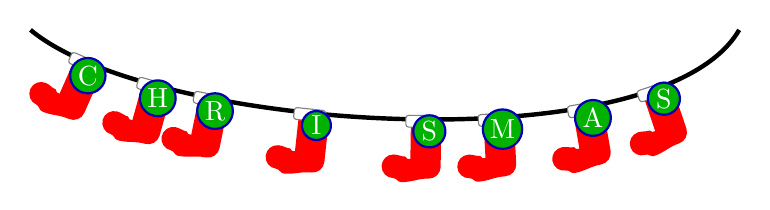
\begin{tikzpicture}[
   mainPicture/.pic = {
      \fill [red] (0,0) -- (0.3,0) -- (0.3,-0.6)
         arc [start angle = 0, delta angle = -90, radius = 0.15]
         to [out = 180, in = 0] (-0.2,-0.8)
         to [out = 180, in = 0] (-0.3,-0.75)
         arc [start angle = 270, delta angle = -180, radius = 0.15]
         to [out = 0, in = 180] (-0.15,-0.475)
         arc [start angle = 200, delta angle = 90, radius = 0.05]
         |- cycle;
      \fill [white, draw = gray, thin, rounded corners = 1pt]
         (-0.15,-0.1) rectangle (0.25,0.05);
      \node at (0.15,-0.15) [
         circle,
         fill = green!70!black,
         text=white,
         draw = blue!70!black,
         thick,
         inner sep = 1pt,
      ] {#1};
   }
]
   \draw [ultra thick, black]
      (0,0) .. controls +(-40:2) and +(240:2) .. (9,0)
      foreach \position / \Bild in {%
         0.1/C,0.2/H,0.3/R,0.4/I,0.5/S,
         0.6/M ,0.7/A,0.8/S%
      } {
         pic [pos = \position +0.02 *rand, sloped]
           {mainPicture=\Bild}
        };
        

\end{tikzpicture}
\end{document}